\section{Week 5 - Chapter D: Diffusion}

\subsection{D.1 Intro + Diffusion Equation}

\begin{defbox}{Diffusion}
Transport of mass (small particles, molecules, dye) in a fluid \textit{without} macroscopic flow.
\end{defbox}

\begin{notebox}[Remarks]
\begin{itemize}
    \item Diffusion and convective transport often happen simultaneously.
    \item Chemical diffusion (mass transport) is mathematically analogous to thermal conduction.
\end{itemize}
\end{notebox}

\subsubsection{D.1.1 Micro Description of Diffusion}

\paragraph{Model: Random Walk on a 1D Lattice}
Let $n(x,t)$ be the number density of particles at position $x$ at time $t$. Let $\Delta x$ be the lattice spacing.

\begin{center}
\begin{tikzpicture}[scale=1.5]
    \draw[thick, ->] (0,0) -- (6,0) node[right] {$x$};
    \foreach \x/\l in {1/{x-\Delta x}, 3/{x}, 5/{x+\Delta x}} {
        \filldraw (\x,0) circle (2pt) node[below=0.2] {$\l$};
    }
    \draw[->, thick, primary] (3, 0.2) to[bend left] node[above] {$p$} (5, 0.2);
    \draw[->, thick, accent] (3, 0.2) to[bend right] node[above] {$1-p$} (1, 0.2);
\end{tikzpicture}
\end{center}

Assume a particle jumps left with probability $1-p$ and right with probability $p$. If $p=1/2$, the walk is unbiased; otherwise, it is biased.

To find the change of number density $\Delta n$ in time $\Delta t$, we compute the net flow into position $x$:
\begin{align*}
\text{Inflow} &= n(x+\Delta x, t)(1-p) + n(x-\Delta x, t)p \\
\text{Outflow} &= n(x, t)[p + (1-p)] = n(x, t)
\end{align*}

Thus, the change in density is:
\[
\Delta n \approx \frac{\partial n}{\partial t} \Delta t = n(x+\Delta x, t)(1-p) + n(x-\Delta x, t)p - n(x, t)
\]

Treating $n(x,t)$ as continuous, we perform a Taylor expansion in space up to the second order:
\begin{align*}
n(x+\Delta x, t) &\approx n(x) + \Delta x\frac{\partial n}{\partial x} + \frac{\Delta x^{2}}{2}\frac{\partial^{2}n}{\partial x^{2}} \\
n(x-\Delta x, t) &\approx n(x) - \Delta x\frac{\partial n}{\partial x} + \frac{\Delta x^{2}}{2}\frac{\partial^{2}n}{\partial x^{2}}
\end{align*}

Plugging this into the $\Delta n$ equation yields:
\[
\frac{\partial n}{\partial t} \Delta t = -\Delta x(1-2p)\frac{\partial n}{\partial x} + \frac{\Delta x^{2}}{2}\frac{\partial^{2}n}{\partial x^{2}}
\]

\begin{eqbox}{Convection-Diffusion Equation (1D)}
\[
\frac{\partial n}{\partial t} + v\frac{\partial n}{\partial x} = D\frac{\partial^{2}n}{\partial x^{2}}
\]
where:
\begin{itemize}
    \item $D = \frac{\Delta x^{2}}{2\Delta t}$ is the \textbf{diffusion coefficient} $[m^2/s]$.
    \item $v = (1-2p)\frac{\Delta x}{\Delta t}$ is the \textbf{drift velocity}.
\end{itemize}
\end{eqbox}

For an \textbf{unbiased random walk} ($p = 1/2 \implies v=0$), we recover the standard 1D Diffusion equation:
\[
\frac{\partial n}{\partial t} = D\frac{\partial^{2}n}{\partial x^{2}}
\]

\paragraph{Extension to 3D Lattice}
For an unbiased walk on a 3D Cartesian lattice, the jump probability in any of the 6 directions is $p=1/6$.

\begin{center}
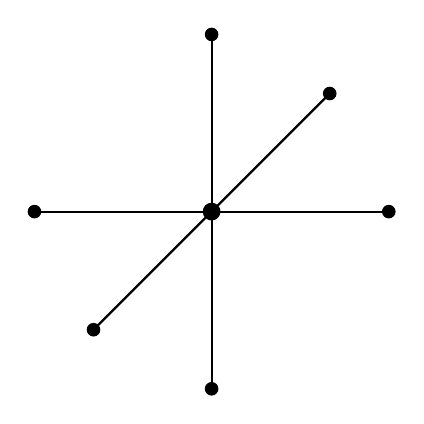
\begin{tikzpicture}[scale=1.5]
    \filldraw (0,0) circle (2pt);
    \draw[thick] (-1.5,0) -- (1.5,0);
    \draw[thick] (0,-1.5) -- (0,1.5);
    \draw[thick] (-1,-1) -- (1,1);
    \filldraw (1.5,0) circle (1.5pt); \filldraw (-1.5,0) circle (1.5pt);
    \filldraw (0,1.5) circle (1.5pt); \filldraw (0,-1.5) circle (1.5pt);
    \filldraw (1,1) circle (1.5pt); \filldraw (-1,-1) circle (1.5pt);
\end{tikzpicture}
\end{center}

Applying the same logic, the equation becomes:
\[
\frac{\partial n}{\partial t} = \frac{\Delta x^{2}}{6\Delta t} \left(\frac{\partial^{2}n}{\partial x^{2}} + \frac{\partial^{2}n}{\partial y^{2}} + \frac{\partial^{2}n}{\partial z^{2}}\right) \implies \frac{\partial n}{\partial t} = D \nabla^{2}n \quad \text{with } D = \frac{\Delta x^{2}}{6\Delta t}
\]

\paragraph{Estimating Diffusion Coefficients}
\begin{itemize}
    \item \textbf{Self-diffusion} (Kinetic theory): $D \sim \frac{1}{6}\delta \left(\frac{3k_{B}T}{m}\right)^{1/2}$
    \item \textbf{Suspended particle} (Stokes-Einstein relation, 1905): $\mathcal{D} = \frac{k_{B}T}{6\pi\mu a}$ for a sphere of radius $a$ in a liquid with dynamic viscosity $\mu$.
\end{itemize}

---

\subsubsection{D.1.2 Continuum Description}
Let $C(\vec{x},t)$ be the macroscopic concentration field (units: $\frac{1}{m^3}$ or $\frac{\text{mol}}{m^3}$).
Observation: Molecules diffuse from high to low concentration.

\begin{defbox}{Fick's First Law}
The particle flux $\vec{j}$ (number of molecules transported through an area per unit time) is proportional to the negative gradient of the concentration:
\[
\vec{j} = -D\nabla C
\]
\end{defbox}

\paragraph{Mass Conservation}
Consider a fixed control volume $V$ bounded by a surface $S$. The rate of change of mass inside must equal the net flux through the surface:
\begin{center}
\begin{tikzpicture}
    \draw[thick] (0,0) ellipse (2.5cm and 1.8cm);
    \node at (0,0) {\Large $V$};
    \node at (1.8,1.4) {$S$};
    \draw[thick, ->, >=stealth] (2.5,0) -- (3.8, 0.6) node[right] {$\hat{n}$};
    \draw[thick, accent, ->, >=stealth] (2.5,0) -- (4, -0.2) node[right] {$\vec{j}$};
\end{tikzpicture}
\end{center}

\[
\frac{d}{dt}\int_{V}C \, dV = -\oint_{S} \vec{j} \cdot d\vec{S}
\]
Using Gauss's Divergence Theorem on the right-hand side:
\[
-\oint_{S} \vec{j} \cdot d\vec{S} = -\int_{V} \nabla \cdot \vec{j} \, dV
\]
For an arbitrary volume $V$, this implies the differential form of mass conservation:
\[
\frac{\partial C}{\partial t} + \nabla \cdot \vec{j} = 0
\]

\begin{eqbox}{The Diffusion Equation}
Substituting Fick's Law ($\vec{j} = -D\nabla C$) into the conservation equation, assuming constant $D$:
\[
\frac{\partial C}{\partial t} = D\nabla^{2}C
\]
\end{eqbox}

\begin{notebox}[Boundary Conditions]
To solve this PDE, appropriate initial and boundary conditions are needed:
\begin{itemize}
    \item \textbf{Dirichlet (Fixed Concentration):} $C(\text{surface}) = C_0$
    \item \textbf{Neumann (Fixed Flux):} $-D \hat{n} \cdot \nabla C = j_0$
    \item \textbf{Robin (Mixed/Convective):} $j = h(C - C_{\infty})$ where $h$ is a mass transfer coefficient.
\end{itemize}
\end{notebox}

---

\subsection{D.2 Solving the Diffusion Equation (Steady State)}

In a steady state, the concentration profile does not change with time, meaning $\frac{\partial C}{\partial t} = 0$. The diffusion equation simplifies to Laplace's equation: $\nabla^{2}C = 0$.

\subsubsection{Example 1: 1D Thin Pipe}
\begin{center}
\begin{tikzpicture}
    \draw[->, thick] (-0.5,0) -- (5,0) node[right] {$x$};
    \draw[->, thick] (0,-0.5) -- (0,3.5) node[above] {$C(x)$};
    \draw[thick, primary] (-0.5, 0.8) -- (0,0.8) node[left] {$\alpha$};
    \draw[thick, accent] (0,0.8) -- (4,2.8);
    \draw[thick, primary] (4,2.8) -- (5,2.8) node[right] {$\beta$};
    \draw[dashed] (4,0) node[below] {$L$} -- (4,2.8);
    \draw (0,0) circle (2pt);
\end{tikzpicture}
\end{center}
Governing ODE: $D\frac{d^{2}C}{dx^{2}} = 0 \implies C(x) = A_{1}x + A_{2}$.
Applying Boundary Conditions $C(0) = \alpha$ and $C(L) = \beta$:
\[
A_2 = \alpha, \quad A_1 = \frac{\beta - \alpha}{L} \implies C(x) = \frac{\beta - \alpha}{L}x + \alpha
\]
\textit{Note: The concentration profile is independent of $D$ in 1D steady state, but the steady flux depends on $D$: $j = -D \frac{\beta-\alpha}{L}$.}

\subsubsection{Example 2: 3D Spherical Shell}
\begin{center}
\begin{tikzpicture}
    \draw[thick] (0,0) circle (1.2cm);
    \draw[thick] (0,0) circle (3cm);
    \draw[->, thick] (0,0) -- (1.2,0) node[midway, above] {$R_1$};
    \draw[->, thick] (0,0) -- (0,-3) node[midway, right] {$R_2$};
    \draw[->, accent, thick, >=stealth] (4.5, 0) -- (3, 0) node[midway, above, text=black] {Inward flux $\vec{j}$};
\end{tikzpicture}
\end{center}

In spherical coordinates with purely radial dependence, the steady-state equation is:
\[
\frac{1}{r^{2}}\frac{d}{dr}\left(r^{2}\frac{dC}{dr}\right) = 0
\]
Integrating twice gives the general solution:
\[
r^{2}\frac{dC}{dr} = A_{1} \implies \frac{dC}{dr} = \frac{A_1}{r^2} \implies C(r) = -\frac{A_{1}}{r} + A_{2}
\]

\textbf{Applying Boundary Conditions:}
1. Inner boundary (Fixed concentration): $C(R_{1}) = 0 \implies A_{2} = \frac{A_{1}}{R_{1}}$
2. Outer boundary (Fixed inward flux $\alpha$): $D\frac{dC}{dr}\Big|_{R_{2}} = \alpha \implies D\frac{A_{1}}{R_{2}^{2}} = \alpha \implies A_{1} = \frac{\alpha R_{2}^{2}}{D}$

Substituting $A_1$ and $A_2$ back into the general solution:
\begin{resultboxnamed}{Radial Concentration Profile}
\[
C(r) = \alpha\frac{R_{2}^{2}}{D}\left(\frac{1}{R_{1}} - \frac{1}{r}\right)
\]
\end{resultboxnamed}

\begin{center}
\begin{tikzpicture}
    \draw[->, thick] (0,0) -- (5,0) node[right] {$r$};
    \draw[->, thick] (0,0) -- (0,3.5) node[above] {$C(r)$};
    \draw[dashed] (1.5,0) node[below] {$R_1$} -- (1.5,3);
    \draw[dashed] (4,0) node[below] {$R_2$} -- (4,3);
    \draw[thick, primary, domain=1.5:4, samples=50] plot (\x, {3.5 * (1/1.5 - 1/\x)});
\end{tikzpicture}
\end{center}